\documentclass{article}
\usepackage[T1]{fontenc}
\usepackage{iclr2026_conference,times}
\input{math_commands.tex}
\usepackage{amsmath,amssymb,booktabs,float,graphicx,microtype,multirow,placeins,tabularx}
\usepackage[hidelinks]{hyperref}
\usepackage{url}

\title{Is Data Value Path-Ordered or Set-Ordered?\\A Carrier-Dependent Same-Sample Test Under WSD Schedules}
\author{Anonymous authors}

\begin{document}
\maketitle

\begin{abstract}
Data attribution is usually indexed by a selected set even when optimization follows a schedule.
We test whether marginal value changes with a target's entry position by measuring the same target
at multiple positions within each seed. On two frozen synthetic logistic carriers, the paired
estimator gives different readings: the registered sine carrier has a negative departure
($g=-0.186$, 95\% CI $[-0.258,-0.115]$), whereas the linear carrier is ambiguous
($g=+0.010$, CI $[-0.112,+0.132]$). The paired sign must not be conflated with the
cross-sectional Kendall sign: negative $g$ means that moving the same target earlier lowers its
value, while negative cross-sectional $\tau$ ranks earlier-scheduled targets higher. A pure
set-ordered ridge counter-arm reveals a non-negative estimator bias ($g=+0.102$, CI
$[+0.028,+0.176]$ on the canonical allocation; positive point estimates on all four allocations).
The canonical allocation therefore fires the sealed two-sided binary contract, but the positive
bias cannot generate the negative sine departure; no magnitude correction is transported across
carriers. Value-conditioned routing also reproduces the cross-sectional B2 signal in a set-ordered
world. The study thus provides a controlled, carrier-dependent measurement, not a general decision
between path-ordered and set-ordered value.
\end{abstract}

\section{Introduction}
Set-indexed attribution methods predict model behavior from training-set membership
\citep{ilyas2022datamodels,park2023trak}, but they do not retain the path by which samples entered
optimization. This abstraction leaves a prior measurement question: is per-sample marginal value
invariant to entry order? If it is, an order-invariant attribution can summarize sample ranking. If
it is not, the same sample set can induce different marginal-value relations under different entry
schedules.

Distinguishing these cases requires more than a nonzero correlation. The entry construction must be
explicit; the seed, rather than the item, must be the inference unit; a minimum effect must be
separated from statistical significance; and the estimator must be measured on a known set-ordered
case. We implement this contract in a deterministic logistic-regression bed. The same sample
identities and held-out readout are evaluated under three entry rules, using both a path-sensitive
leave-one-out value and an order-invariant comparator.

The result has three parts. First, same-sample pairing prevents a cross-sectional selection signal
from being read as a path effect. Second, the sine carrier shows a negative paired departure while
the linear carrier remains ambiguous. Third, the set-ordered ridge counter-arm exposes a
non-negative paired-estimator bias, and a separate routing experiment shows that B2 is a
reference-conditioned stress test. These results are limited to two synthetic carriers.

\begin{figure}[t]
\centering
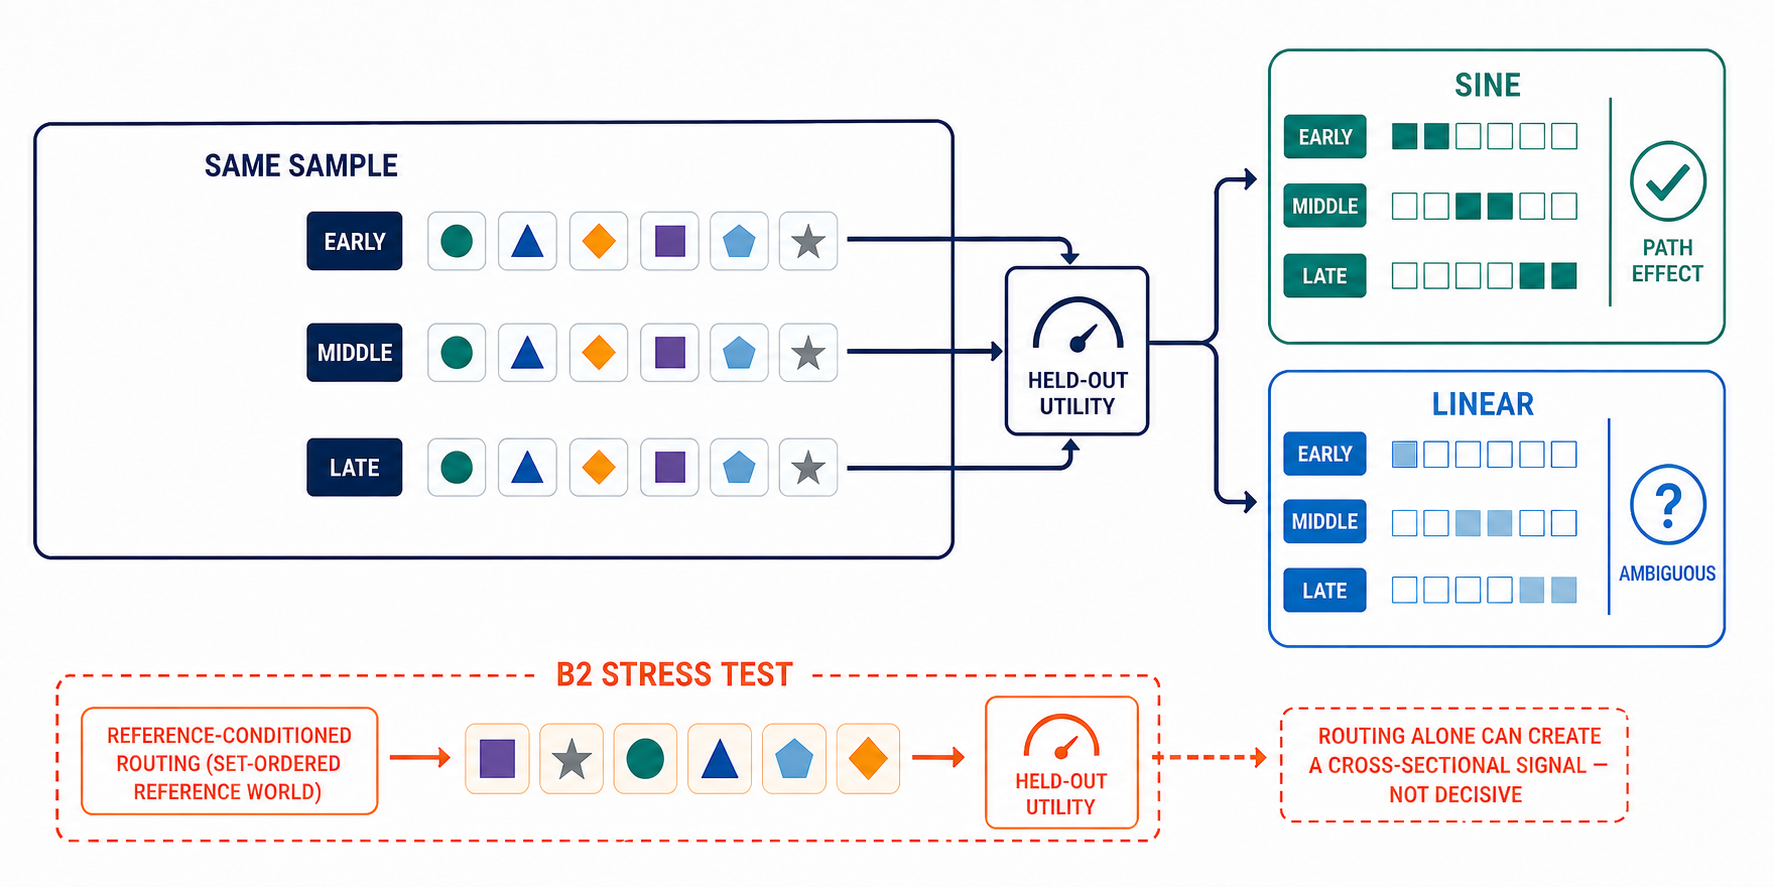
\includegraphics[width=0.95\linewidth]{figures/figure1.png}
\caption{Qualitative measurement schematic extracted from the supplied frozen PDF. Each target is
measured at early, middle, and late entry while identity and held-out readout remain fixed. The B2
lane is separate because reference-conditioned routing can create a cross-sectional signal in a
set-ordered world. The schematic contains no experimental values.}
\label{fig:schematic}
\end{figure}

\section{Problem and Estimands}
For seed $k$, let $D_k$ be the clean training set, $G_k$ a fixed target set, and $H_k$ a fixed
held-out split. Entry construction $c$ assigns each target $z\in G_k$ a schedule location $s_c(z)$.
With $U(w;H_k)$ denoting held-out negative cross-entropy (higher is better), define empirical path
value as
\begin{equation}
V_{c,k}(z)=U\!\left(w_{c,k}^{+G};H_k\right)-U\!\left(w_{c,k}^{-z};H_k\right),
\label{eq:path-value}
\end{equation}
where both fits use the same WSD budget and differ by leaving out target $z$. The seed-level path
statistic is
\begin{equation}
\tau_{c,k}=\operatorname{KendallTau}\!\left(\{s_c(z)\}_{z\in G_k},
\{V_{c,k}(z)\}_{z\in G_k}\right).
\label{eq:path-tau}
\end{equation}
Negative $\tau$ means that earlier-scheduled targets rank higher in held-out marginal value. We
average Equation~\ref{eq:path-tau} across seeds and form frozen 95\% Student-$t$ intervals over
seed-level coefficients. A two-sided Wilcoxon signed-rank test corroborates paired constructions.
The minimum meaningful magnitude is $\tau_a=0.10$.

We report a cell as \emph{null} when its interval includes zero, \emph{sig-sub-threshold} when the
interval excludes zero but remains inside the magnitude boundary, \emph{sig-supra-threshold} when
the entire interval lies beyond the boundary in the effect direction, and \emph{reverse} for a
significant reversal. The separate field \texttt{exceeds\_threshold} records the magnitude decision.

On the same $D_k\cup G_k$ and $H_k$, the order-invariant comparator fits a regularized logistic
model and evaluates the inverse-Hessian leave-one-out approximation
\begin{equation}
V_{\mathrm{set},k}(z)=-\nabla_w U(w_k^*;H_k)^\top H_k^{-1}g_k(z),
\label{eq:set-value}
\end{equation}
where $H_k$ is the regularized training Hessian and $g_k(z)$ is the target-sample loss gradient.
This is the operational GLM reduction used here, not an implementation of the full TRAK or
datamodel pipelines.

\section{Frozen Experimental Design}
The experiment uses two 24-dimensional synthetic logistic carriers. The linear carrier contains a
clean class-separated pool and conflicting near-duplicates with flipped labels. The second carrier,
retained under the frozen key \emph{sine}, uses a shifted Gaussian pool with a fixed linear label
boundary; targets negate the first feature and flip the label. The key therefore does not imply
general nonlinear coverage.

\begin{table}[t]
\centering\small
\caption{Frozen experimental contract. Items within a seed are not independent inference units.}
\label{tab:contract}
\begin{tabularx}{\linewidth}{@{}lX@{}}
\toprule
Component & Frozen setting \\
\midrule
Carriers & linear; registered sine carrier \\
Dimension / pool & $d=24$; 400 clean examples per seed \\
Split / targets & 320 clean train; 80 held out; 40 conflicting targets \\
Optimizer & full-batch logistic GD; $\ell_2$ coefficient $10^{-3}$ \\
WSD budget & $T=300$; 10\% warmup, 80\% stable, 10\% decay \\
Entry locations & $0.15T$, $0.50T$, $0.85T$ (rank-linear positions for B1) \\
Inference & 16 seeds; per-seed Kendall $\tau$; 95\% Student-$t$ CI \\
Magnitude gate & $\tau_a=0.10$ \\
Negative control & 20 seeded trials; Bonferroni/FWER-controlled detector \\
\bottomrule
\end{tabularx}
\end{table}

\paragraph{Entry constructions.}
Construction A inserts the complete target block from one of the three schedule locations onward
and computes leave-one-out value within that block. B1 assigns each target a distinct injection step
spread from $0.15T$ to $0.85T$. B2 ranks targets by the fixed set-valued reference, partitions the
order into thirds, and injects high-, middle-, and low-ranked regions at the early, middle, and late
locations. Thus B1 changes per-sample position, whereas B2 also couples reference rank to entry
time. The comparison identifies the entry rule, not merely whether position changed.

For Construction A and $t\in\{0.15T,0.50T,0.85T\}$, targets outside the chosen block have
$s_A(z)=0$ and targets inside it have $s_A(z)=\lfloor tT\rfloor$. Both leave-one-out fits retain the
same WSD budget, matching Equation~\ref{eq:path-value}.

\paragraph{Controls and frozen decision.}
The clean negative control is a strictly convex quadratic ridge substrate with additive,
schedule-invariant influence. Independent random position labels use a per-seed critical value
Bonferroni-adjusted over 20 trials; the frozen acceptance condition is no fires. A global
construction-dependent verdict requires the threshold-crossing pattern to vary by construction or
carrier and does not license a universal mechanism claim. The six cells, seeds, and analysis rules
were frozen before the writing pass.

\section{Construction Sensitivity}
\begin{figure}[t]
\centering
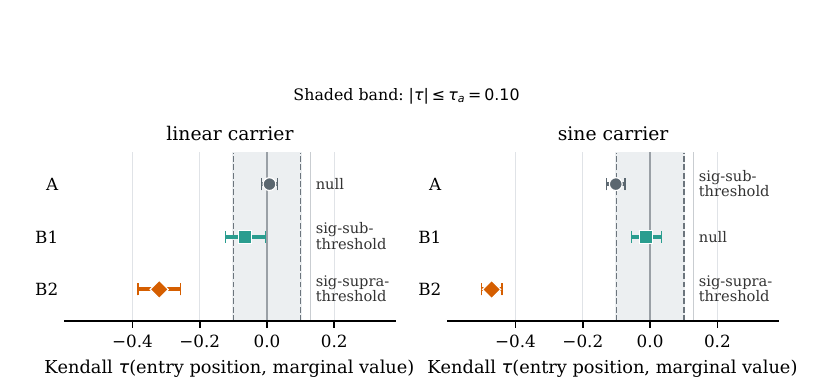
\includegraphics[width=0.95\linewidth]{figures/figure2.png}
\caption{Frozen six-cell construction sensitivity (16 seeds per cell), extracted from the supplied
PDF. Points are mean per-seed Kendall $\tau$; bars are 95\% Student-$t$ intervals; the shaded band is
$|\tau|\le\tau_a=0.10$. Exact values appear in Table~\ref{tab:six-cell}.}
\label{fig:six-cell}
\end{figure}

\begin{table}[t]
\centering\footnotesize
\caption{Frozen six-cell result. Only B2 crosses the magnitude boundary on both carriers. Intervals
are per-cell and unadjusted; they are not treated as six independent tests.}
\label{tab:six-cell}
\setlength{\tabcolsep}{3.5pt}
\begin{tabular}{lllclc}
\toprule
Carrier & Construction & $\tau$ & 95\% CI & Four-state label & Exceeds \\
\midrule
linear & A: block & $+0.007$ & $[-0.017,+0.032]$ & null & false \\
linear & B1: rank-linear & $-0.065$ & $[-0.125,-0.005]$ & sig-sub-threshold & false \\
linear & B2: region-lumped & $-0.321$ & $[-0.384,-0.257]$ & sig-supra-threshold & true \\
sine & A: block & $-0.102$ & $[-0.130,-0.075]$ & sig-sub-threshold & false \\
sine & B1: rank-linear & $-0.011$ & $[-0.056,+0.033]$ & null & false \\
sine & B2: region-lumped & $-0.471$ & $[-0.502,-0.440]$ & sig-supra-threshold & true \\
\bottomrule
\end{tabular}
\end{table}

Cross-sectionally, B2 lies beyond $-\tau_a$ on both carriers, whereas A and B1 do not. Statistical
significance alone would give a different headline: sine A and linear B1 exclude zero but remain
below the minimum-effect threshold. Because B2 value-conditioned routing can reproduce this pattern
on a set-ordered world, the paired analysis below is load-bearing.

\subsection{Construction-axis separation}
The frozen interval comparison separates B2 from A and B1 on both carriers. A and B1 overlap on
linear by 0.011 but are separated on sine. These within-cell interval comparisons are descriptive;
direct inference uses within-seed contrasts.

\begin{table}[t]
\centering\scriptsize
\caption{Frozen construction-axis interval comparison.}
\label{tab:axis}
\begin{tabularx}{\linewidth}{@{}lXXX@{}}
\toprule
Pair & linear & sine & Composite \\
\midrule
B2 vs A & separated: $[-.384,-.257]$ vs $[-.017,.032]$ & separated: $[-.502,-.440]$ vs $[-.130,-.075]$ & both \\
B2 vs B1 & separated: $[-.384,-.257]$ vs $[-.125,-.005]$ & separated: $[-.502,-.440]$ vs $[-.056,.033]$ & both \\
A vs B1 & overlap 0.011 & separated: $[-.130,-.075]$ vs $[-.056,.033]$ & mixed \\
\bottomrule
\end{tabularx}
\end{table}

The six paired contrasts share the same 16 seeds and form one correlated family. Raw $p$ values
are retained; Bonferroni $\alpha/6=0.0083$ leaves the four B2-involving contrasts significant, while
the two B1--A values straddle that threshold.

\begin{table}[t]
\centering\footnotesize
\caption{Same-seed construction contrasts. ``Beyond'' means the paired CI lies strictly outside
$[-0.10,+0.10]$.}
\label{tab:paired-constructions}
\begin{tabular}{lrrrc}
\toprule
Carrier, pair & $\Delta\tau$ & 95\% CI & $p$ & Beyond \\
\midrule
linear, B2$-$A & $-0.328$ & $[-0.395,-0.260]$ & $3\times10^{-8}$ & yes \\
linear, B2$-$B1 & $-0.256$ & $[-0.325,-0.186]$ & $1\times10^{-6}$ & yes \\
linear, B1$-$A & $-0.072$ & $[-0.124,-0.021]$ & $0.009$ & no \\
sine, B2$-$A & $-0.369$ & $[-0.421,-0.317]$ & $2\times10^{-10}$ & yes \\
sine, B2$-$B1 & $-0.460$ & $[-0.509,-0.411]$ & $3\times10^{-12}$ & yes \\
sine, B1$-$A & $+0.091$ & $[+0.041,+0.141]$ & $0.001$ & no \\
\bottomrule
\end{tabular}
\end{table}

\subsection{Same-sample paired identification}
Cross-sectional $\tau$ is not decisive because B2 routes high-reference-value samples early. We
therefore move each target between $0.15T$ and $0.85T$ while holding every other target at its
frozen B2 step. With $\Delta(z)=V(0.15T;z)-V(0.85T;z)$, define
\begin{equation}
g_k=\frac{\operatorname{mean}_{z\in G_k}\Delta(z)}
{\operatorname{std}_{z\in G_k}\Delta(z)},
\label{eq:paired-g}
\end{equation}
where the denominator uses the 40 targets with \texttt{ddof}=1. Negative $g$ means early entry
lowers the same target's value. This interpretation is opposite to negative cross-sectional $\tau$,
which ranks earlier-scheduled targets higher; the two signs are never equated.

\begin{table}[t]
\centering\small
\caption{Frozen same-sample paired identification (16 seeds).}
\label{tab:paired-id}
\begin{tabularx}{\linewidth}{@{}lXXX@{}}
\toprule
Carrier & Paired slope & Four-state reading & Routing robustness \\
\midrule
sine & $-0.186$, CI $[-0.258,-0.115]$; Wilcoxon $p=9\times10^{-5}$ & PATH-SUPPORTED-neg; early entry lowers value & placebo $g=-0.176$ \\
linear & $+0.010$, CI $[-0.112,+0.132]$; Wilcoxon $p=0.74$ & AMBIGUOUS; not identified & --- \\
\bottomrule
\end{tabularx}
\end{table}

The sine paired departure survives routing permutation and reverses, rather than reproduces, the
cross-sectional sign interpretation. Linear remains unidentified. A per-seed sign-consistency
fraction is omitted because, under this construction, it reduces to bookkeeping with no test power;
an earlier selection-confound claim based on a sign-consistency code bug is revoked.

\subsection{Set-ordered ridge counter-arm}
The identical paired estimator is run on a strictly convex set-ordered ridge whose marginal value is
order-invariant by construction. The sealed contract intended a 16-seed CI covering zero to count
as silent and any CI excluding zero to count as a fire.

\begin{table}[t]
\centering\footnotesize
\caption{Set-ordered ridge calibration and allocation sweep. The sine row is shown only as the
headline reference.}
\label{tab:ridge}
\begin{tabular}{lrrrc}
\toprule
Substrate / allocation & $g$ & 95\% CI & Wilcoxon $p$ & Covers 0 \\
\midrule
ridge, canonical $X_s[0{:}40]$ & $+0.102$ & $[+0.028,+0.176]$ & $0.011$ & no (fires) \\
ridge, $X_s[40{:}80]$ & $+0.192$ & $[+0.130,+0.254]$ & $0.00015$ & no (fires) \\
ridge, $X_s[80{:}120]$ & $+0.049$ & $[-0.066,+0.165]$ & $0.298$ & yes \\
ridge, random slice & $+0.145$ & $[+0.065,+0.225]$ & $0.006$ & no (fires) \\
sine headline & $-0.186$ & $[-0.258,-0.115]$ & $9\times10^{-5}$ & no \\
\bottomrule
\end{tabular}
\end{table}

The canonical ridge allocation literally fires the sealed binary rule. Across all four allocations,
however, point estimates are positive; 14 of 16 canonical seeds are positive, and dropping the most
extreme seed of either sign preserves the positive direction. The contract's sign-blind consequence
clause is therefore an erratum: a positive set-ordered bias cannot produce the negative sine
departure. This is a sign-only conservative argument. We do not subtract the ridge magnitude from
the sine value because cross-carrier transport is untested.

\subsection{B2 as a reference-conditioned stress test}
On the set-ordered ridge, routing targets with the real B2 reference correlations reproduces the
frozen cross-sectional magnitudes; at zero correlation, $\tau$ is near zero.

\begin{table}[t]
\centering\small
\caption{B2 routing stress test (16 seeds).}
\label{tab:b2-stress}
\begin{tabular}{lrrrr}
\toprule
Carrier & operating $\rho$ & routing-only $\tau$ & frozen B2 $\tau$ & zero-corr. $\tau$ \\
\midrule
linear & $0.30$ & $-0.313$ & $-0.321$ & $-0.054$ \\
sine & $0.55$ & $-0.563$ & $-0.471$ & $-0.054$ \\
\bottomrule
\end{tabular}
\end{table}

Thus B2 is a reference-conditioned stress test, not standalone path evidence. The paired reading
remains subject to the ridge calibration above.

\section{Set-Valued Baseline and Bed Certificate}
On the same carriers, targets, splits, and constructions, we compute mean within-construction
Kendall agreement $\tau_{AB}$ between empirical path value and Equation~\ref{eq:set-value}.
Because frozen uncertainty intervals are unavailable, these values are descriptive.

The detector controls separate aliveness, power on a known path effect, and false alarms on a known
set-ordered substrate.

\begin{table}[H]
\centering\footnotesize
\caption{Detector calibration. Family sizes are explicit because the unadjusted and FWER-controlled
rates use different trial counts.}
\label{tab:detector}
\begin{tabularx}{\linewidth}{@{}Xrrr@{}}
\toprule
Control & Family & Fires & Rate \\
\midrule
Decoupled positive control (schedule dependence independent of B2 score) & 16 seeds & 14 & 87.5\% \\
Order-invariant negative, unadjusted $\alpha=0.05$ & 100 trials & 3 & 3\% \\
Order-invariant negative, frozen FWER control & 20 trials & 0 & 0\% (SILENT) \\
\bottomrule
\end{tabularx}
\end{table}

\begin{table}[H]
\centering\small
\caption{Descriptive agreement with the set-valued comparator.}
\label{tab:agreement}
\begin{tabular}{lcc}
\toprule
Carrier & B1 rank-linear & B2 region-lumped \\
\midrule
linear & $+0.20$ & $+0.30$ \\
sine & $+0.57$ & $+0.55$ \\
\bottomrule
\end{tabular}
\end{table}

\begin{table}[H]
\centering\footnotesize
\caption{Frozen bed-discriminability certificate. B2 fires as a routing-sensitive probe but is not
the known-path positive control.}
\label{tab:certificate}
\begin{tabularx}{\linewidth}{@{}Xcc@{}}
\toprule
Reading & linear & sine \\
\midrule
Known-path decoupled positive control & $14/16$ (87.5\%) & $14/16$ (87.5\%) \\
B2 routing-sensitive stress probe & $\tau=-0.321$ & $\tau=-0.471$ \\
Known-set negative-control fires & $0/20$ SILENT & $0/20$ SILENT \\
Set estimator alive (fraction distinct) & $1.0$ & $1.0$ \\
Live $\tau_{AB}$ aliveness read & $+0.88$ & $+0.72$ \\
Verdict & DISCRIMINATING & DISCRIMINATING \\
\bottomrule
\end{tabularx}
\end{table}

No single probe is certified on all three properties. The paired arm, not B2, supplies the evidence
for entry-position sensitivity.

\FloatBarrier
\section{Related Work}
Datamodels and TRAK are indexed by selected sets rather than schedule position
\citep{ilyas2022datamodels,park2023trak}. Our narrower question is whether empirical leave-one-out
value has a schedule-dependent component when identities and held-out readout remain fixed.
Machine-learning conclusions can be sensitive to power, run variance, and reporting choices
\citep{card2020power,bouthillier2021variance,dodge2019show,reimers2017reporting}; we therefore use
seeds as inference units and separate confidence against zero from a minimum-effect decision.
Training-trajectory suites motivate treating schedules as first-class experimental objects
\citep{biderman2023pythia}, and the frozen analysis follows the rationale for preregistration in NLP
\citep{vanmiltenburg2021preregistering}.

\section{Limitations and Scope}
The evidence is limited to deterministic CPU logistic-regression carriers with synthetic conflicts;
the registered sine key does not represent general nonlinear models or language models. The paired
test is primary, while B2 is a routing-reproducible stress test. Its set-ordered calibration has a
non-negative bias, and the canonical allocation fires the sealed two-sided rule; only the sign-based
conservative conclusion is supported. Linear is not identified. The comparator is an
inverse-Hessian GLM reduction, not end-to-end TRAK or datamodels, and its agreement values lack
frozen uncertainty. A single set-ordered negative control cannot exclude every artifact or calibrate
natural data. Transfer requires a natural carrier, fresh controls, full same-bed baselines, and
agreement uncertainty.

\section{Conclusion}
The same-sample paired test gives carrier-dependent readings: the sine carrier has a negative
departure ($g=-0.186$, CI $[-0.258,-0.115]$) whose meaning reverses the cross-sectional sign,
whereas the linear carrier is ambiguous ($g=+0.010$, CI $[-0.112,+0.132]$). The set-ordered ridge
counter-arm has non-negative bias across four allocations, so it cannot explain the negative sine
departure, but the canonical allocation fires the sealed sign-blind binary rule and no cross-carrier
magnitude correction is justified. Because routing reproduces the B2 cross-sectional signal on a
set-ordered world, B2 remains a stress test. These synthetic results do not decide whether data value
is generally path-ordered or set-ordered.

\FloatBarrier
\label{p5:main-text-end}
\bibliographystyle{iclr2026_conference}
\bibliography{refs}

\appendix
\section{Reproducibility and Disclosure}
All runs reported in the supplied manuscript are deterministic CPU experiments with the seed as the
statistical unit. The quantitative plot is reproduced here by a faithful extraction from the supplied
frozen PDF because the exact historical LaTeX and plotting source were unavailable. Generative
tooling assisted language and typesetting; no generated asset created or modified quantitative
evidence. The study uses synthetic data and no human participants or personal information.

\section{Frozen Provenance}
The supplied PDF maps the following artifacts by SHA-256 prefix; this editorial pass transcribes but
does not independently execute them.
\begin{description}\small
\item[\texttt{61894856}] R127 order run: \texttt{candidateB\_order\_r127.json}
\item[\texttt{2e08b7f9}] R126 reconcile: \texttt{candidateB\_reconcile\_r126.json}
\item[\texttt{3a1c18da}] R128 four-state labels: \texttt{candidateB\_relabel\_4state\_R128.json}
\item[\texttt{3178724b}] R128 bed certificate: \texttt{candidateB\_bed\_discriminability\_R128.json}
\item[\texttt{40b74cbc}] R133 construction CI: \texttt{candidateB\_construction\_axis\_CI\_R133.json}
\item[\texttt{d74eb619}] R127 preregistration supplement.
\item[\texttt{d0c898fb}] R126 preregistration draft.
\item[\texttt{547978c5}] R139 same-sample paired and placebo artifact.
\item[\texttt{b7028282}] R140 rebuild (re-frozen R214).
\item[\texttt{f6ba5097}] R140 rebuild specification.
\item[\texttt{502c13bf}] R141 preregistration, revision 2.
\item[\texttt{67c52c0b}] R141 stress test and routing placebo.
\item[\texttt{e3431b7f}] R148 set-ordered ridge counter-arm preregistration.
\item[\texttt{6b437ba5}] R148 counter-arm output, canonical allocation.
\item[\texttt{397dd466}] R148 counter-arm code.
\item[\texttt{b81168c4}] R148 counter-arm finding record, including the allocation sweep.
\end{description}

\end{document}
